\documentclass{article}
\usepackage{graphicx} % Required for inserting images
\makeatother
\setcounter{secnumdepth}{4} 
\setcounter{tocdepth}{4}
\begin{center}
\title {\textbf{ Blood Bank Management Systems (Android Apps)}}
\author 
{\textbf{Submitted By}\\ Name: Rakibur Rahman Id:19201103082\\ Name: Eyamin Molla Id:19202103209\\ Name:MdMohibbullah Id:19201103101\\ Name: Nahian Islam Id:19201103028\\ Name:MD Shahadat Hasan Rakib Id:19202103304\\
\textbf{Submitted To}\\ Mr. Sudipto Chaki (Assistant Professor)\\
Dept of CSe
Bangladesh University of Business and
Technology 
}
\date{April 2023}
\end{center}
\begin{document}



\maketitle
\newpage
\tableofcontents
\newpage
\section{Introduction}
The Blood Bank App is an Android-based mobile application that provides a platform for blood
donors and recipients to connect with each other. The app offers a simple and user-friendly
interface for users to register themselves as blood donors or search for blood donors in their
area. The need for an efficient and accessible platform for blood donation and request
management is crucial in addressing the challenges faced in the healthcare domain. The existing
processes often suffer from communication gaps, delays in accessing blood units during
emergencies, and difficulties in connecting potential donors with recipients. The Blood Bank App
project aims to overcome these challenges by leveraging the power of mobile technology. It seeks
to create a user-friendly platform that promotes blood donation, enables efficient blood request
management, and facilitates timely responses during critical situations. Blood donation is a
crucial service that saves millions of lives every year. However, finding blood donors during
emergencies can be a challenging task, especially in remote areas. The Blood Bank App aims to
bridge this gap by providing a digital platform where donors and recipients can easily connect
with each other. Some of the key features of the Blood Bank App include creating a donor profile,
searching for blood donors based on location and blood type, sending blood requests to donors,
and receiving real-time updates on the status of the request. The app also allows donors to
update their availability status, view their donation history, and receive notifications on
upcoming blood donation camps in their area. The app is designed to be secure, user-friendly,
and salable, with the potential to expand its services to other healthcare initiatives. Overall, the
Blood Bank App is a much-needed solution that leverages technology to streamline blood
donation and improve accessibility to blood donors for those in need.
\section{Objective}
The objective of the Blood Bank App project is to develop an Android-based mobile application
that facilitates the process of blood donation and blood requests. To create awareness about the
importance of blood donation and encourage individuals to become blood donors. To provide a
user-friendly platform for blood banks, hospitals and individuals to efficiently request and
manage blood requirements. Enabling users to check availability of blood units at nearby blood
banks and connect with potential donors in real-time. Establish a comprehensive donor
management system that allows easy registration, profile creation and communication with
registered blood donors. Facilitating rapid response to emergency situations by notifying
registered donors immediately of urgent blood requirements in their vicinity. Using GPS
technology to identify the location of donors and blood banks, which makes it easier to connect
donors with recipients based on proximity. Implementing strong security measures to ensure the
privacy of user information, maintaining privacy throughout the app.
Creating a user-friendly interface for individuals to register as blood donors, create and manage
their profiles and update their availability status. Collaborating with blood banks and healthcare
institutions to integrate their databases into the app, ensure real-time updates on blood
availability and facilitate seamless blood requests. Incorporating GPS technology to track users'
location and display nearby blood banks, hospitals and donors on a map for quick access and
effective communication. Implement a notification system that alerts registered users to blood
requests, emergencies and relevant updates, improving response time and overall efficiency.
Integrating a feedback mechanism into the app for users to rate their donation experience,
provide suggestions and report any issues, encouraging continuous improvement. Develop
analytical tools to generate insights into blood donation trends, user engagement and areas for
improvement, enabling data-driven decision making and strategic planning. Incorporate strong
security protocols to protect user data, ensure compliance with privacy regulations, and build
trust among users. By fulfilling these objectives and goals, the Blood Bank App will serve as a
valuable tool in connecting blood donors and recipients, promoting timely response to
emergencies and ultimately saving lives.
\section{Motivation}
The motivation behind developing the Blood Bank App as an Android-based mobile application
stems from the critical need for an efficient and accessible platform to address the challenges
faced in blood donation and request management. The existing processes often lack streamlined
communication, leading to delays in accessing blood units during emergencies and difficulty in
connecting potential donors with recipients. By leveraging the widespread use of smartphones
and the convenience of mobile applications, the Blood Bank App aims to bridge this gap and
revolutionize the way blood donation is carried out The Blood Bank app aims to increase the
number of available donors and simplify the process of connecting them with recipients,
ultimately reducing blood shortages and saving lives. In critical situations such as accidents or
surgery, quick access to blood units is crucial. The app's real-time availability feature and instant
notifications to nearby donors ensure quick response. Traditional methods of blood request
management often involve manual processes and coordination challenges. The Blood Bank app
simplifies the process, making it more efficient by using technology to seamlessly connect donors
and recipients. The app serves as a platform to create awareness about the importance of blood
donation and encourage more individuals to participate in this life-saving act. It aims to educate
the community about the impact of blood donation in saving lives and building a culture of
regular blood donation. With increasing smartphone penetration, creating an Android-based
blood bank app allows for greater reach and accessibility. People can easily download and use
the app on their mobile devices, increasing convenience and participation. The app incorporates
robust security measures to protect user information and maintain privacy. Addressing privacy
concerns to build trust among users, ensuring their participation and willingness to share their
personal information
\section{Project Futures}

The Blood Bank App, developed as an Android-based mobile application, encompasses several
key features that contribute to its effectiveness in blood donation and request management.
These features include:
\begin{itemize}
    \item User Registration and Profile Creation: The app allows individuals to register as
blood donors, providing their relevant information such as blood type, contact
details, and availability for donation. Users can create and manage their profiles
within the app.
    \item Blood Request Management: Users can submit blood requests through the app,
specifying the required blood type, quantity, and urgency. The app efficiently
manages these requests, ensuring they reach nearby blood donors and blood
banks promptly.
\item Real-time Blood Availability: The app provides real-time updates on blood
availability in nearby blood banks. Users can check the availability of specific blood
types and locate the nearest blood banks where the required blood units are in
stock.
\item Location-Based Services: Leveraging GPS technology, the app identifies the
location of users and displays nearby blood banks, hospitals, and donors on a map.
This feature enables users to easily locate and connect with potential donors or
blood banks.
\item Notification System: The app incorporates a notification system to instantly alert
registered blood donors about urgent blood requests or emergency situations in
their vicinity. Notifications are sent directly to their mobile devices, ensuring a
quick response.
\item Donor-Recipient Communication: The app facilitates seamless communication
between blood donors and recipients. Users can initiate conversations, exchange
relevant information, and coordinate the logistics of blood donation or collection
through secure messaging within the app.
\item Donation History and Reminders: The app keeps track of a user's donation history,
providing a record of their past contributions. It also sends reminders to users
about their eligibility for blood donation based on predefined intervals and
criteria.
\item Feedback and Rating: The app includes a feedback mechanism that allows users
to rate their donation experiences, provide feedback, and offer suggestions for
improvement. This feature promotes continuous enhancement of the app's
functionalities.
\end{itemize}
These project features collectively contribute to the effectiveness and efficiency of the Blood
Bank App, providing a user-friendly platform for blood donation promotion, streamlined blood
request management, and timely responses during emergencies.
\section{Project Development Stages}
The Agile methodology is a way to manage a project by breaking it up into several phases. It involves constant collaboration with stakeholders and continuous improvement at every stage. Once the work begins, teams cycle through a process of planning, executing, and evaluating.
\begin{figure}[h]
    \centering
    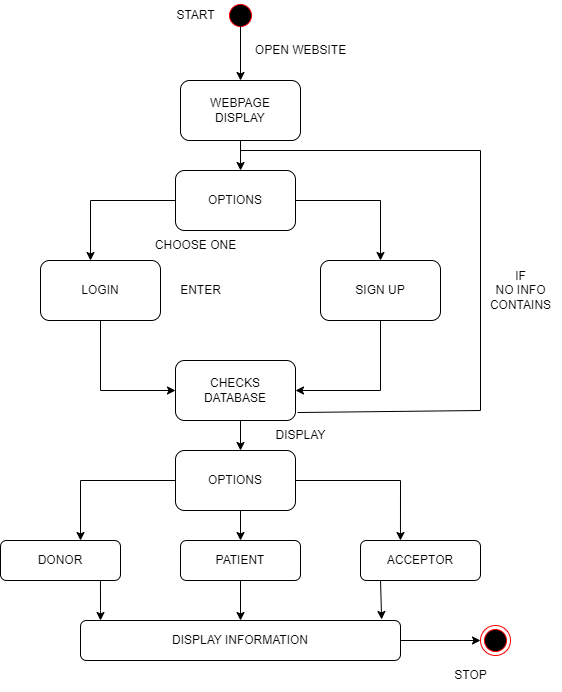
\includegraphics[ width=6cm]{img/gi.png}
    \caption{Blood Bank Andorid apps}
    \label{fig:enter-label}
\end{figure}
\begin{enumerate}
    \item Project planning and research.
    \item User interface design and wire-framing.
    \item Database design and development.
    \item Integration of Google Maps API for location-based search.
    \item User authentication and authorization setup.
    \item Implementation of the donor profile management system.
    \item Integration of push notifications for blood donation requests.
    \item Testing and debugging.
\end{enumerate}
\section{Current limitations}
While the Blood Bank App project aims to address various challenges in blood donation and
request management, it is essential to acknowledge the current limitations of the application.
One of the challenges faced by the app is ensuring widespread user adoption. Encouraging
individuals to download, register, and actively use the app requires extensive marketing efforts
and awareness campaigns to reach a large user base. The app heavily relies on internet
connectivity for real-time updates, notifications, and data exchange. In areas with limited or
unstable internet access, users may face difficulties in using the app effectively. The app's
effectiveness is dependent on the participation of blood banks and registered donors. In regions
with a limited number of blood banks or a low number of registered donors, the app's ability to
connect users with available blood units may be constrained. Building trust among users
regarding the accuracy of information, donor authenticity, and privacy of personal data is crucial.
Implementing robust verification mechanisms and addressing concerns related to data security
are ongoing challenges. The app's effectiveness in connecting donors and recipients relies on a
comprehensive database of blood banks and donors. Ensuring broad geographical coverage,
especially in remote areas or underdeveloped regions, can be challenging. While the Blood Bank
App project aims to mitigate these limitations through continuous improvements and updates, it
is essential to acknowledge and address these challenges to ensure the app's long-term
effectiveness and success.
\section{Future Works}
In terms of future works, the Blood Bank App has the potential for further development and
enhancement. One possible area for improvement is the incorporation of more advanced
features such as machine learning algorithms to optimize blood donor matching, or digital wallets
for seamless transactions between blood donors and recipients. Additionally, the app could be
expanded to include a feature for tracking blood donation history and incentivizing frequent
donors through rewards and recognition programs. Another potential area for development is
the integration of social media platforms into the app, allowing for easier sharing of blood
donation opportunities with a wider audience. With continued investment and innovation, the
Blood Bank App has the potential to make a meaningful impact on blood donation practices and
ultimately save lives.
\section{Conclusion}
The development of the Blood Bank App represents a significant step forward in streamlining
blood donation practices and improving access to life-saving resources. Through its user-friendly
interface and intuitive design, the app has the potential to attract a larger pool of blood donors
and simplify the process of finding and receiving necessary blood transfusions. While there is still
much room for improvement and expansion, the success of this project highlights the power of
technology in addressing real-world challenges and promoting positive social change. With
continued support and investment, the Blood Bank App has the potential to revolutionize the
way we approach blood donation.



\end{document}
